\documentclass[169,xcolor=table]{beamer}

\usetheme{ccc}

\usepackage{polyglossia}
\usepackage{csquotes}
\usepackage{fontspec}
\usepackage{blindtext}
\usepackage{graphicx}
\usepackage{listings}
\usepackage{appendixnumberbeamer}
\usepackage{tikz}
\usepackage{pifont}
\usepackage{booktabs}
\usepackage{changepage}
\usetikzlibrary{positioning}
\usetikzlibrary{arrows.meta}
\usetikzlibrary{shapes.geometric}
\usetikzlibrary{calc}
\usetikzlibrary{fit}
\usetikzlibrary{graphs}
\usetikzlibrary{matrix}
\usepackage{upquote}
\usepackage{biblatex}

\definecolor{lightgray}{gray}{0.9}

\addbibresource{zotero.bib}

\lstset{upquote=true}
%\setsansfont[BoldFont={Fira Sans SemiBold}]{Fira Sans Book}
\makeatletter
\newlength\beamerleftmargin
\setlength\beamerleftmargin{\Gm@lmargin}
\makeatother

\title{Learning Vulnerability Discovery with Global-Relational Models}
\subtitle{Research Project Compiler Construction}
\author{Benno Fünfstück}
\date{October 7, 2021}

\begin{document}

%\includeonlyframes{current}

\tikzset{
  onslide/.code args={<#1>#2}{%
    \only<#1>{\pgfkeysalso{#2}}% \pgfkeysalso doesn't change the path
  },
  temporal/.code args={<#1>#2#3#4}{%
    \temporal<#1>{\pgfkeysalso{#2}}{\pgfkeysalso{#3}}{\pgfkeysalso{#4}}%
  },
  hidden/.style = {opacity=0},
  uncover/.style = {temporal=#1{hidden}{}{hidden}},
  drawalert/.style = {temporal=#1{}{color=alerted text.fg}{}}
}

\newcounter{tmlistings}

\newcommand\makenode[2]{%
  \tikz[baseline=0pt, remember picture] { \node[fill=gray!50,thick,rounded corners,anchor=base,#1/.try] (listings-\the\value{tmlistings}) {{\scriptsize\the\value{tmlistings}} #2}; }%
  \stepcounter{tmlistings}%
}

\maketitle

\begin{frame}\frametitle{Deep learning for vulnerability detection}
  \begin{tabular}{lrrr}
    \toprule
    Metrics & µVuldeepecker & Lin et al. & {\bfseries POEM} \\
    \midrule
    C Accuracy & 80.0\% & 88.0\% & \bfseries{90.9\%} \\
    C FPR      & 31.6\% & 30.5\% & \bfseries{3.1\%} \\
    C FNR      & 9.4\%  & \bfseries{7.1\%}  & 8.9\% \\
    \bottomrule
  \end{tabular}

  \fullcite{ye_deep_2020}

  (Dataset: ``collected from standard vulnerable code databases'')
\end{frame}

\begin{frame}<1>[label=overall]\frametitle{Overall structure: binary classification of functions}
  \begin{tikzpicture}
    \matrix[row sep=20pt, nodes={minimum width=80pt, inner ysep=5pt}] (layers) {
      \node       (inp) {input sample}; \\
      \node[draw,drawalert=<2>] (emb) {initialisation}; \\
      \node[draw,drawalert=<3>] (rep) {model}; \\
      \node[draw,drawalert=<4>] (ext) {output}; \\
      \node       (out) {prediction}; \\
    };

    \node[above right=10pt and 70pt of rep, text width=130pt] (seq-rnn) {sequence-based RNN};
    \node[right=10pt and 70pt of rep, text width=130pt] (graph-ggnn) {graph-based GGNN \cite{li_gated_2017}};
    \node[below right=10pt and 70pt of rep, text width=130pt] (combined-sandwich) {sandwich model \cite{hellendoorn_global_2019}};

    \node[right=70pt of inp] (functions) {\bfseries functions};
    \node[right=70pt of out,text width=95pt] (vuln) {\bfseries \hfill not vulnerable (0)\\ \hfill vulnerable (1)};

    \graph { (inp) -> (emb) -> (rep) -> (ext) -> (out) };

    \draw[dashed]
      (rep.east) -- (seq-rnn.north west) -- ({$(combined-sandwich.south east)$} |- {$(seq-rnn.north east)$}) -- (combined-sandwich.south east) -- (combined-sandwich.south west) -- cycle;
    \draw[dashed, <-] (inp) -- (functions);
    \draw[dashed, ->] (out) -- (vuln);
  \end{tikzpicture}
\end{frame}


\begin{frame}\frametitle{Are sandwich models better for vulnerability prediction?}
  \begin{exampleblock}{Goal}
    Evaluate the sandwich model from Hellendoorn et al. on the task of vulnerability detection
  \end{exampleblock}

  \begin{enumerate}
    \item Implement in Compy-Learn~\cite{brauckmann_compy-learn_2020}
    \item Review existing datasets for ML vulnerability discovery
    \item Evaluate the model on \emph{real world data}
  \end{enumerate}
\end{frame}

\section{Model}

\begin{frame}[fragile]\frametitle{A sample function}

\begin{lstlisting}[language=C, morekeywords={uint8_t},
  emph={buf}, emphstyle=\color{green!60!black},
  emph={[2]out}, emphstyle={[2]\color{blue!90!black}},
  emph={[3]pkt_len}, emphstyle={[3]\color{cyan!80!black}},
  emph={[4]i}, emphstyle={[4]\color{alert}},
]
int decode_packet(char *buf, char *out) {
  uint8_t pkt_len = buf[0];
  for (int i = 0; i < pkt_len; ++i) {
    out[i] = buf[i + 1];
  }
  return pkt_len;
}
\end{lstlisting}

  \vspace{10pt}

  \begin{tikzpicture}[
    keyword/.style = {font=\bfseries},
    buf/.style = { text=green!60!black },
    uncover=<2->
    ]
    \matrix[matrix of nodes, column sep=5pt, row sep=20pt, ampersand replacement=\&, nodes={
      draw, minimum height=20pt, anchor=north, text height=10pt, text depth=3pt,
    }] {
      |[keyword] (n0)|int \& |(n1)| decode\_packet \& |[inner xsep=23pt] (n2)| ( \& |[keyword] (n3)|char \& |[inner xsep=10pt] (n4)| * \& |[buf] (n5)|buf \& |[draw=none]| {\large$\cdots$}  \\
    };
    \node[anchor=north west, inner xsep=0pt] at (n0.south west) { int };
    \node[anchor=north west, inner xsep=0pt] at (n1.south west) { identifier };
    \node[anchor=north west, inner xsep=0pt] at (n2.south west) { l\_paren };
    \node[anchor=north west, inner xsep=0pt] at (n3.south west) { char };
    \node[anchor=north west, inner xsep=0pt] at (n4.south west) { star };
    \node[anchor=north west, inner xsep=0pt] at (n5.south west) { identifier };

  \end{tikzpicture}
\end{frame}

\begin{frame}[t]\frametitle{Recurrent Neural Networks (RNN)}
  \begin{tikzpicture}[
    keyword/.style = {font=\bfseries},
    buf/.style = { text=green!60!black },
    ]
    \matrix[matrix of nodes, column sep=5pt, row sep=0pt, ampersand replacement=\&, nodes={
      draw, minimum height=20pt, anchor=north, text height=10pt, text depth=3pt,
    }] {
      |[keyword] (n0)|int \& |(n1)| decode\_packet \& |[inner xsep=23pt] (n2)| ( \& |[keyword] (n3)|char \& |[inner xsep=10pt] (n4)| * \& |[buf] (n5)|buf \& |[draw=none]| {\large$\cdots$}  \\
      |[draw=none]| int   \& |[draw=none]| identifier \& |[draw=none]| l\_paren \& |[draw=none]| char \& |[draw=none]| star \& |[draw=none]| identifier \& \\
    };

    % \node[anchor=north west, inner xsep=0pt] at (n0.south west) { int };
    % \node[anchor=north west, inner xsep=0pt] at (n1.south west) { identifier };
    % \node[anchor=north west, inner xsep=0pt] at (n2.south west) { l\_paren };
    % \node[anchor=north west, inner xsep=0pt] at (n3.south west) { char };
    % \node[anchor=north west, inner xsep=0pt] at (n4.south west) { star };
    % \node[anchor=north west, inner xsep=0pt] at (n5.south west) { identifier };


  \end{tikzpicture}
\end{frame}

\begin{frame}\frametitle{Representation as Graph: augmented AST}
\end{frame}

\begin{frame}\frametitle{Gated Graph Neural Networks (GGNN)}
\end{frame}

\begin{frame}\frametitle{Extraction: Global Attentation}
\end{frame}

\begin{frame}\frametitle{Sandwich models: Combining GGNNs and RNNs}
\end{frame}

\begin{frame}\frametitle{Batching for sandwich models}
\end{frame}


\section{Data}

\begin{frame}\frametitle{A real world vulnerability (National Vulnerability Database)}
  \only<1>{
  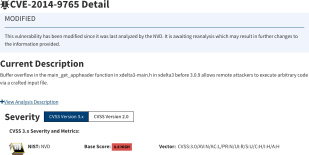
\includegraphics[width=\framewidth]{media/cve-2014-summary}
  }
  \only<2>{
  \includegraphics[width=\framewidth]{media/cve-2014-ref}
  }
  \only<3>{
  \includegraphics[width=\framewidth]{media/xdelta-commit}
  }
\end{frame}

\begin{frame}[fragile]\frametitle{The bug}
  \begin{adjustwidth}{-0.5em}{-1.5em}
  \begin{lstlisting}[numbers=left, language=C, emph={parsed}, emphstyle={\alert}, emph={[2]place}, emphstyle={[2]\color{brown!60!black}}]
xd3_get_appheader (stream, & apphead, & appheadsz);

char *start = (char*)apphead;
char *slash;
int   place = 0;
char *parsed[4];
memset (parsed, 0, sizeof (parsed));

while ((slash = strchr (start, '/')) != NULL) {
  *slash = 0;
  parsed[place++] = start;
  start = slash + 1;
}
  \end{lstlisting}
  \end{adjustwidth}
\end{frame}

\begin{frame}\frametitle{Existing datasets}
  % diversity
  % label precision
  % size
  % naturalness
  \rowcolors[]{1}{}{lightgray}
  \begin{tabular}{p{11em}p{15em}}
    \toprule
    name & description \\
    \midrule
    SARD/SATE & synthetic, by CWE, originally for testing static analyzers \\
    Draper \cite{russell_automated_2018} & code from Debian/GitHub, labels from static analyzer \\
    Devign \cite{zhou_devign_2019} & ffmpeg/qemu commits filtered by keyword and manual review \\
    ReVeal \cite{chakraborty_deep_2020}& CVEs from debian, labels mined from git diff \\
    \bottomrule
  \end{tabular}
\end{frame}

\begin{frame}[label=current]\frametitle{Challenge 1: compilation}
  \begin{tikzpicture}
    \def\lwidth{0.1pt};
    \begin{scope}[local bounding box=samples]
     \def\corner{0.15in};
     \def\cornerradius{0.02in};
     \def\h{1.7cm};
     \def\w{2cm};
     \foreach \i in {0,1,2} {
     \coordinate (nw) at ($(-0.05in*\i,-0.06in*\i)$);
     \coordinate (ne0) at ($(nw) + (\w, 0)$);
     \coordinate (ne1) at ($(ne0) - (\corner, 0)$);
     \coordinate (ne2) at ($(ne0) - (0, \corner)$);
     \coordinate (se) at ($(ne0) + (0, -\h)$);
     \filldraw [-, line width = \lwidth, fill=white] (nw) -- (ne1) -- (ne2)
     [rounded corners=\cornerradius]--(se) -- (nw|-se) -- cycle;
     \draw [-, line width = \lwidth] (ne1) [rounded corners=\cornerradius]-- (ne1|-ne2) -- (ne2);
     }
     \node[anchor=north west,node distance=0] at (-0.05in,-0.8) {Samples};
    \end{scope}

    \matrix[above right=1em and 1em of samples, column sep=0pt, ampersand replacement=\&] (debian) {
      \node[anchor=center] {\includegraphics[width=2em]{media/debian-openlogo-nd}}; \& \node[anchor=base]{Deb. Package}; \\
    };

    % \begin{scope}[local bounding box=compiling, below left=1em of debian]
    %   \foreach \angle in {0, 60, ..., 360} {
    %     \draw[fill=black] (0,0) -- (\angle-30:0.7cm) -- (\angle-30+8:0.7cm) -- (\angle-13:1cm) -- (\angle+13:1cm) -- (\angle+30-8:0.7cm) -- (\angle+30:0.7cm) -- cycle;
    %   };
    %   \draw[fill=white] (0,0) circle [radius=0.3];
    % \end{scope}

    \draw[dashed,->] (samples) |- (debian);
  \end{tikzpicture}
\end{frame}

% ReVeal
% Devign
% Draper
% SARD/SATE
%

\begin{frame}\frametitle{Challenge 2: dataset is noisy}
  \includegraphics[width=\framewidth]{media/reveal-unbalanced}
\end{frame}

\section{Results}


\begin{frame}\frametitle{Model can fit the training data}

\end{frame}

\begin{frame}\frametitle{Model does not generalize}
\end{frame}

\begin{frame}\frametitle{Future directions}
  {\bfseries 1. improve embedding}: embed identifier names, simplify graphs \\
  \vspace{4em}
  {\bfseries 2. better dataset}: clean with heuristic, other sources (OSS Fuzz, Joern)
\end{frame}

\begin{frame}\frametitle{Summary}
  \begin{columns}
    \begin{column}{0.5\textwidth}
      \begin{enumerate}
        \item succefully implemented sandwich model using compy learn
        \item no model able to generalize on real world data
        \item real world data is hard to find, need better datasets first
      \end{enumerate}
    \end{column}
    \begin{column}{0.5\textwidth}
      \only<2>{
      \includegraphics[width=0.8\textwidth]{media/bug-captcha}
      }
    \end{column}
  \end{columns}
\end{frame}

\appendix

\begin{frame}[allowframebreaks]{References}
  \printbibliography
\end{frame}


\end{document}
